\documentclass{article}
\usepackage[utf8]{inputenc}
\usepackage{mathrsfs, amsmath, mathbbol, graphicx, amssymb}
    % mathrsfs = símbolos: lagrangiano
        % \mathscr{L}
    % amsmath = romper ecuaciones en nuevas líneas y centrar
        % \begin{split}
        % \end{split}
    % mathbbol = Para mostrar los conjuntos numéricos
    % graphix = Para insertar imágenes
    % amssymb = Para caracterés de operación raros, como equivalente.
\setlength{\parskip}{5px}

\title{Cálculo integral: valor presente y valor futuro}
\author{
    Jorge Antonio Gómez García \\
    Emiliano Martín Lugo López \\
    Saud Antonio Morales González}
\date{22/05/2022}

\begin{document}
\maketitle

\section*{Índice}
    \begin{itemize}

        \item Introducción (no es menciona de forma directa ninguna fórmula de integración): \begin{itemize}
            \item ¿Qué es el valor futuro?
            \item ¿Qué es el valor presente?
            \item Ejemplo (sin explicitar ninguna integral).
            \item Gráfica del ejemplo.
            \item ¿Cómo puede ayudarnos el cálculo integral a resolver este problema?
        \end{itemize}

        \item Entrando en materia... \begin{itemize}
            \item ¿Por qué $e$? (+ anécdota)
            \item Calculando el valor futuro + fórmula general
            \item Calculando el valor presente + fórmula general
            \item Ejemplos (x2).
        \end{itemize}

        \item Ejercicios de Tarea
        
    \end{itemize}

    \section{Introducción. Definición de conceptos y preámbulo al cáluclo integral}

        En este texto, aprenderá una de las aplicaciones más importantes de la integral definida a los negocios negocios y a la economía: el valor presente y futuro. Pero, antes de entrar en materia es necesario que tenga conocimiento de ciertos conceptos básicos que le ayudarán a comprender tanto los problemas de aplicación, como la importancia del uso de las integrales en estos casos.

        \subsection{Interés compuesto}

            Cuando una empresa o una persona obtienen ingresos, pueden decidir si gastarlos en el presente, o invertirlos para obtener intereses en el futuro. +
            Para entender la manera en la que estos agentes toman decisiones con respecto a su dinero, y la manera en la que el dinero genera estos intereses, es necesario que el lector conozca el concepto de \textbf{interés compuesto}:

            \begin{quote}
                Al final de cada periodo, el interés generado durante ese periodo se agrega al capital (monto invertido), de modo que también genere interés en el periodo siguiente. La fórmula básica para el valor (o monto compuesto) de una inversión después de n periodos de interés compuesto es como sigue:
            \end{quote}
            \begin{equation}
                S=P(1+r)^{n}
            \end{equation}

            \begin{quote}
                Para una cantidad de capital ($P$), proporciona el monto de capital compuesto ($S$) a una tasa de interés periódica $r$ al final del $n$ periodos.\footnote[1]{2. pp 97}
            \end{quote}

        \subsection{Flujos de ingreso y anualidades}

            Cuando un agente económico genera un ingreso al realizar una operación económica, podemos decir que tiene un \textbf{flujo de ingreso}, que incluso podrá invertir en el futuro. Así mismo, cuando hablamos del valor futuro del flujo de ingreso, o el flujo futuro, estamos habando del flujo de ingreso inicial sumado al interés que que ha acumulado en un determinado plazo de tiempo.

            Por su parte, las \textbf{anualidades} se determinan como los flujos de ingreso llevados a cabo en determinados periodos de tiempo \textbf{regulares}, dentro de un plazo específico. Un ejemplo de anualidad es el pago de un préstamo automotriz obtenido a crédito.

        \subsection{El valor presente y el valor futuro}

            Ahora bien, conceptos como el \textbf{valor presente} y el \textbf{valor futuro} de una cantidad determinada de inversión, son valores que pueden servirle para determinar la cantidad de dinero que necesita ahorrar para solicitar un crédito de automóvil o un crédito hipotecario, o para saber la cantidad de dinero suficiente necesaria tras un plan de ahorro, como la jubilación.

            \textbf{Valor presente}: Es la manera de asignar valor a cualquier activo de manera que, su cálculo se obtenga de descontar el flujo futuro en base a una tasa de rentabilidad ofrecida por alternativas de inversión comparables denominada tasa mínima.\footnote[2]{3}

            \textbf{Valor futuro}: Este es la cantidad de dinero que una inversión puede alcanzar en una fecha futura al ganar intereses a una tasa compuesta.\footnote[3]{3} Puede darse el caso en el que \textbf{conoce el valor futuro de la inversión, y lo que busca es conocer el valor presente} del capital. Para ello, puede usar la siguiente fórmula:

            \begin{equation}
                P=S(1+r)^{-n}
            \end{equation}

            \begin{quote}
                El capital P que debe invertirse a la tasa periódica r durante n periodos de interés, de modo que el monto total sea S. Este es el \textbf{valor presente} del capital final ($S$).
            \end{quote}

        \subsection{Ejemplos de aplicación previos al cálculo integral}

            \subsubsection{Sobre el valor presente}

                Suponga que depositan \$200 a una cuenta que paga el 8\% de interés compuesto anualmente. Así, usando la ecuación (1) note que la cuenta al final del tercer año valdrá:

                \begin{equation*}
                    200(1.08)^{3} = 251.94
                \end{equation*}

                Describiendo la relación entre el capital inicial y el capital final, podemos decir que este último es el \textit{valor futuro} de los \$200 que, a su vez, son el \textit{valor presente} o capital inicial.

            \subsubsection{Sobre el valor futuro}

                Imagine que debe pagar \$2,000 en tres años, y sabe que la tasa de interés que va a pagar es de 11\% de interés compuesto mensualmente.
                
                Como sabe, La frecuencia de los pagos es mensual, por lo que la cantidad de periodos en la que tiene que dividir sus pagos es de 3 años multiplicado por los meses. Es decir, tiene 36 periodos ($n = 36$). Mientras que la tasa de interés es de 11\% anual. Sin embargo, genera interés compuesto mensualmente, por lo que, usando la ecuación (2) tenemos:

                \begin{equation*}
                \begin{split}
                    P &= 2000 \left(\frac{0.11}{12}\right)^{-3(12)} \\
                    P &\approx 2000(0.0091)^{-36} \\
                    P &\approx 1443.44
                \end{split}
                \end{equation*}

                Una forma gráfica de ver el cálculo del valor presente y del valor futuro es la siguiente:

                \begin{figure}[h]
                    \centering
                    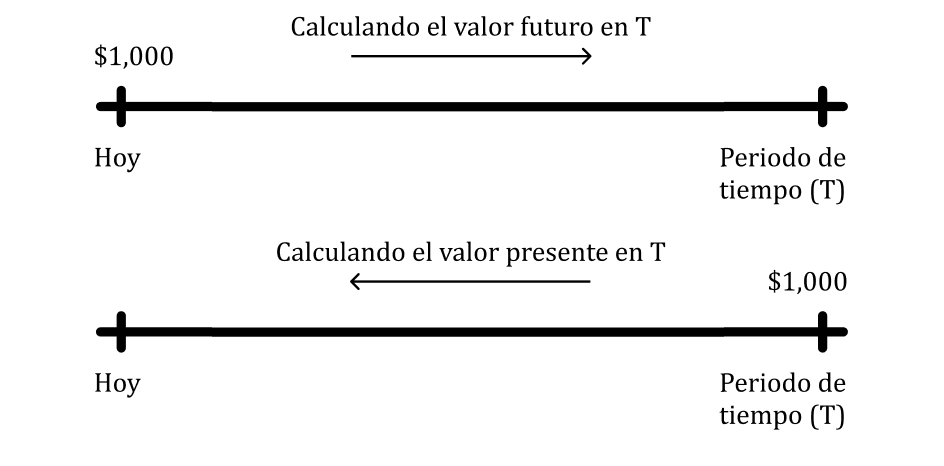
\includegraphics[width=10cm]{img_1.png}
                \end{figure}

        \section{La integral definida y el valor presente y futuro}

        Observe que cuan

            \subsection{¿Por qué $e$?}


            \subsection{Ejemplos de aplicación con cálculo integral}

                \subsubsection{Sobre el valor presente}

                \subsubsection{Sobre el valor futuro}
        \section{Tarea: ejercicios}


\end{document}